\documentclass[tikz,border=10pt]{standalone}
\usetikzlibrary{mindmap}
\begin{document}
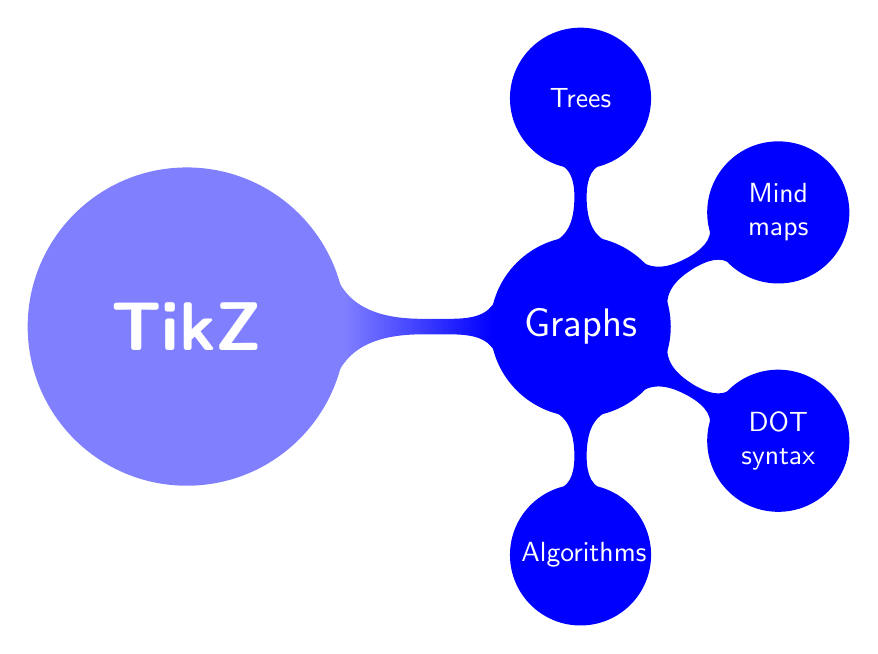
\begin{tikzpicture}[
  mindmap,
  text = white,
  concept color = blue!50,
  nodes = {concept},
  root/.append style = {
    font = \Huge\sffamily\bfseries},
  level 1 concept/.append style =
    {font = \Large\sffamily, sibling angle=90},
  level 2 concept/.append style =
    {font = \normalsize\sffamily}
  ]
  \node [root] {TikZ} [clockwise from=0]
    child [concept color=blue] {
      node {Graphs} [clockwise from=90]
        child { node {Trees} }
        child { node {Mind maps} }
        child { node {DOT syntax} }
        child { node {Algorithms} }
    };
\end{tikzpicture}
\end{document}
